\begin{figure}[!htb]
\centering
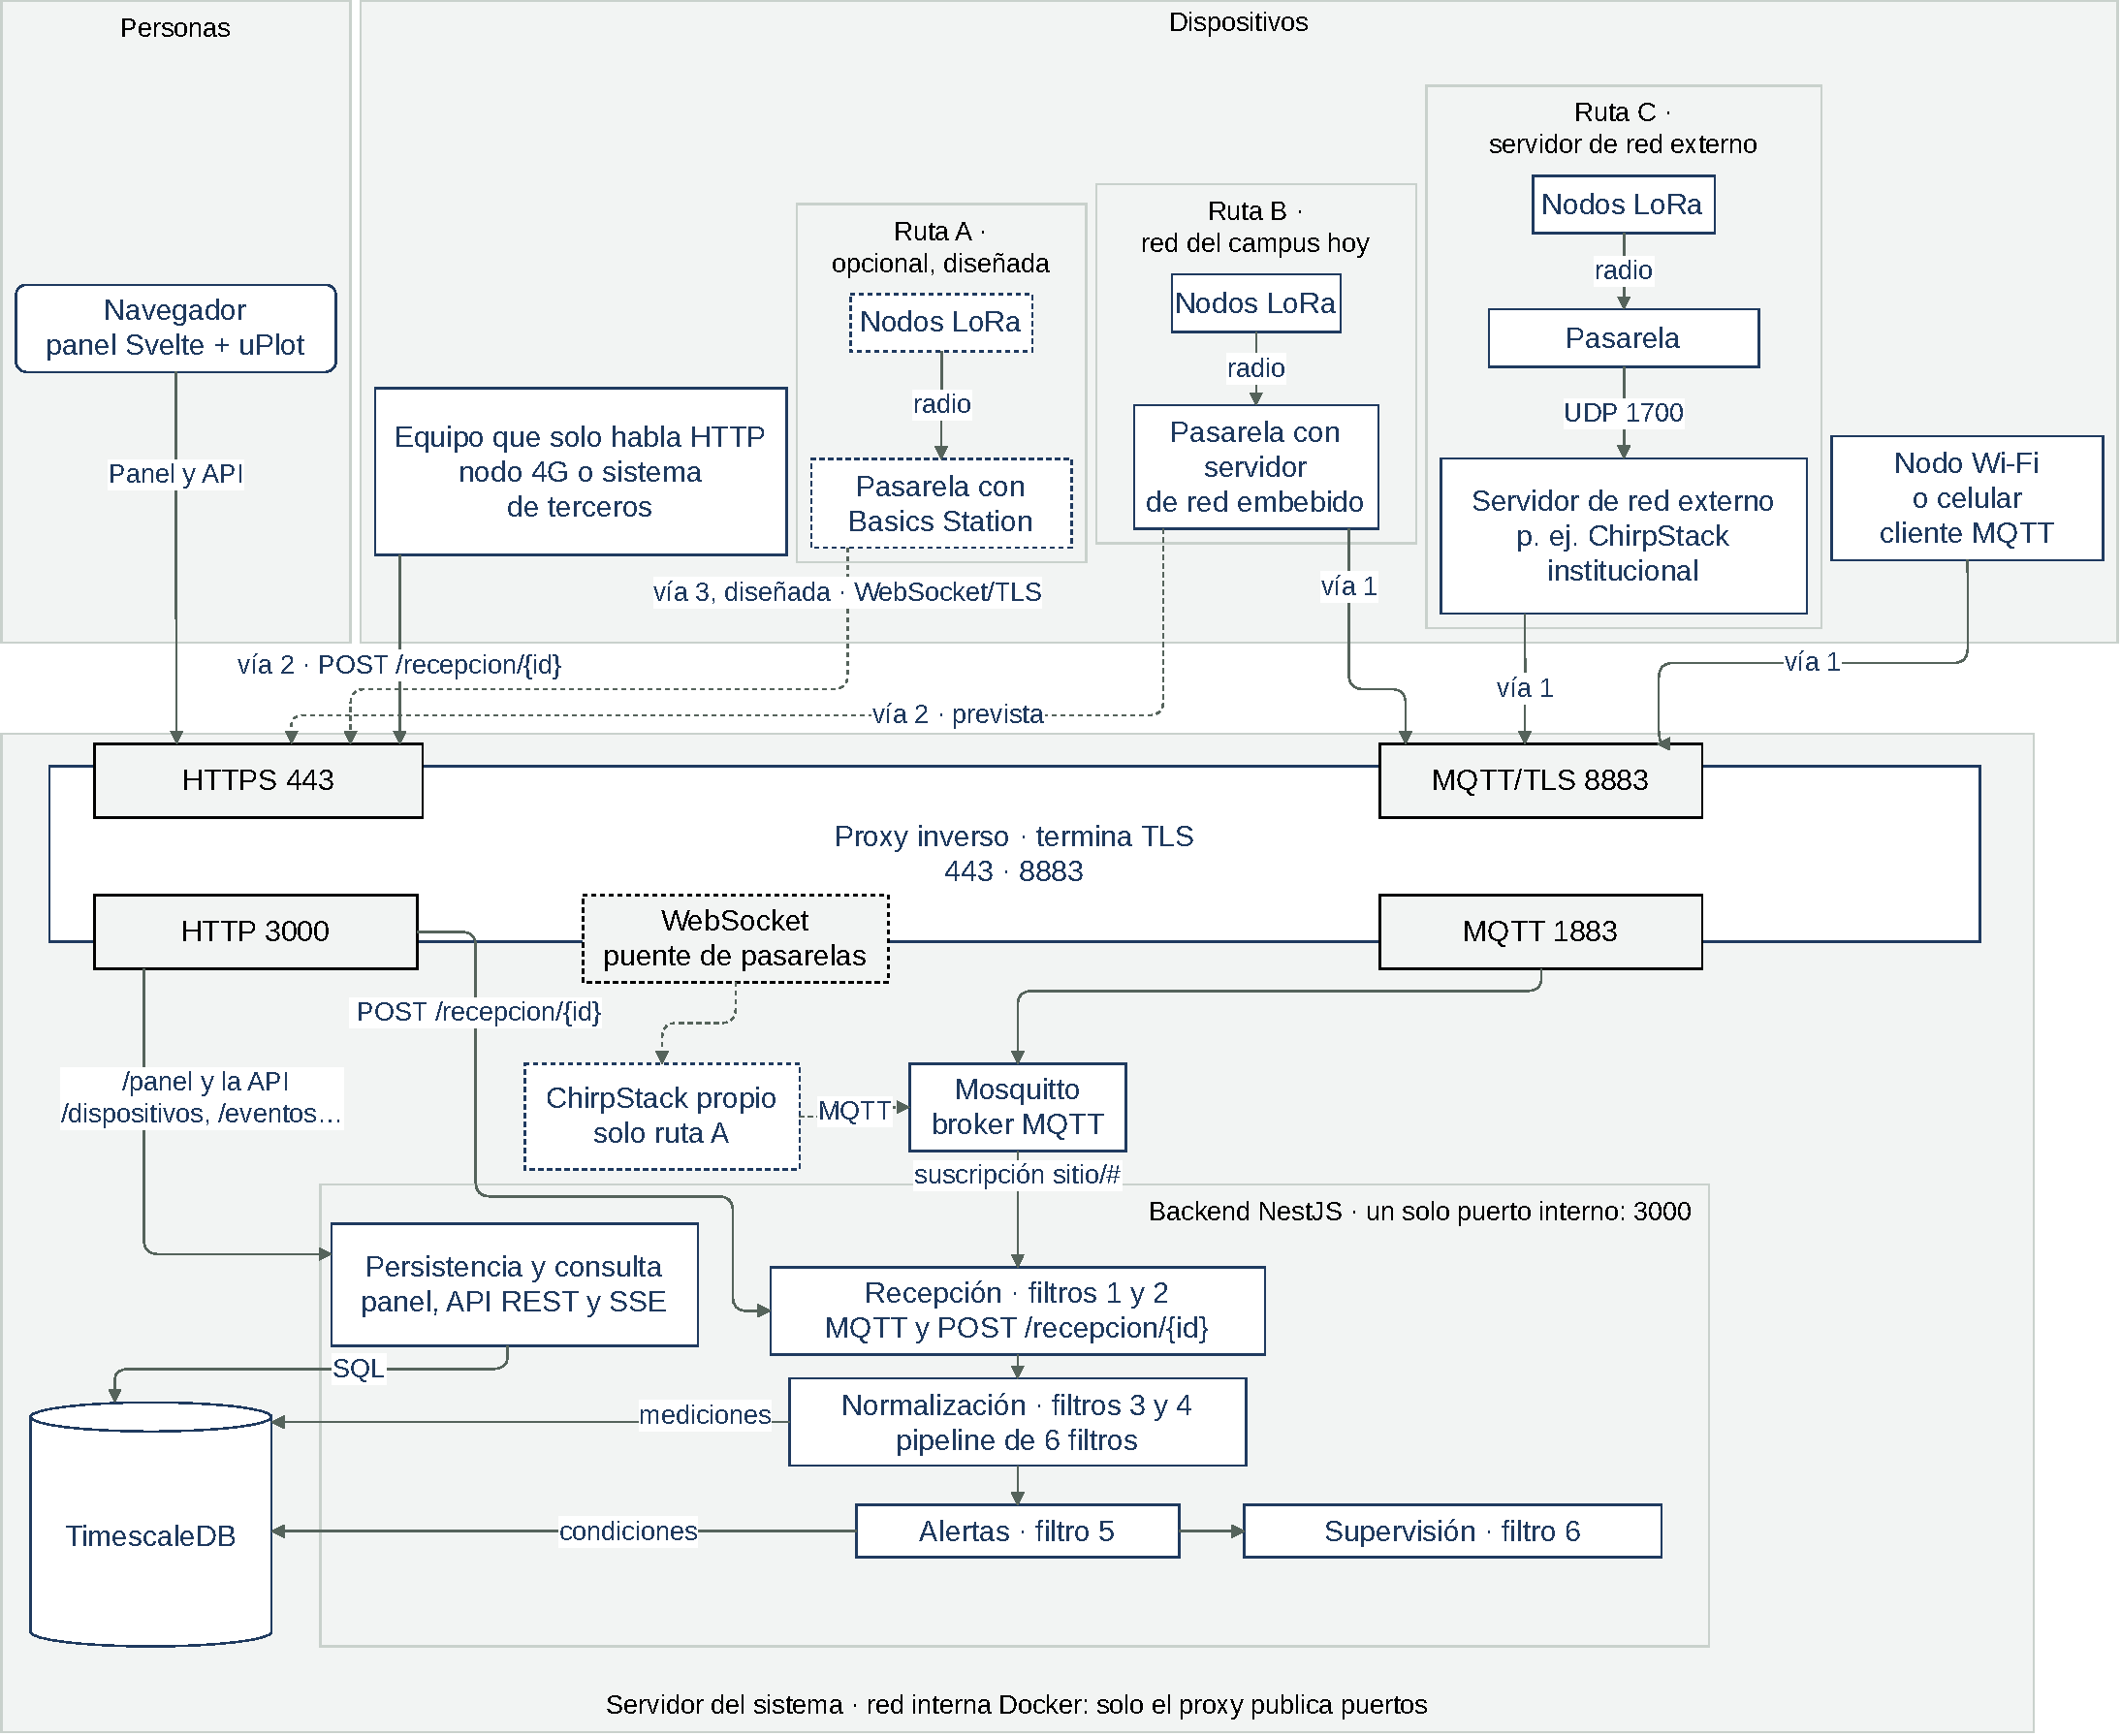
\includegraphics[width=\linewidth,height=0.62\textheight,keepaspectratio]{figuras/drawio/figura-4.1.pdf}
\caption{Vista de contenedores (modelo C4, nivel 2). La frontera del trabajo es el tópico MQTT: de un lado, la red de sensores del compañero (nodos y \emph{gateway}: en la ruta B la pasarela —la red del campus hoy— y en la ruta C un servidor de red externo publican al broker por TLS con su propia credencial (vía 1); en la ruta A, opcional, diseñada y punteada, la pasarela llega por WebSocket sobre TLS con \emph{Basics Station} a un ChirpStack propio (vía 3)); del otro, el proxy —único contenedor expuesto—, el broker y el backend. Un nodo Wi-Fi o celular publica directo por MQTT sobre TLS (vía 1); un equipo que solo habla HTTP entra por 443 con un token (vía 2) y cae en la misma tubería de seis filtros; el reporte HTTPS de la pasarela, variante prevista de la vía 2, va punteado. El navegador nunca se conecta al broker: consume la API del backend, que ya autenticó, validó y normalizó cada trama y, con la sesión de la Etapa 4, cada usuario verá solo los datos de su sitio (RF-41). Las cajas del backend llevan los filtros de la figura~\ref{fig:pipeline} que ejecutan y corresponden a los módulos M1, M2, M6, M4 y M5 del catálogo; M3, M7 y M8 son transversales o viven en el cliente.}
\label{fig:contenedores}
\end{figure}
